\documentclass[twoside]{book}

% Packages required by doxygen
\usepackage{fixltx2e}
\usepackage{calc}
\usepackage{doxygen}
\usepackage[export]{adjustbox} % also loads graphicx
\usepackage{graphicx}
\usepackage[utf8]{inputenc}
\usepackage{makeidx}
\usepackage{multicol}
\usepackage{multirow}
\PassOptionsToPackage{warn}{textcomp}
\usepackage{textcomp}
\usepackage[nointegrals]{wasysym}
\usepackage[table]{xcolor}

% Font selection
\usepackage[T1]{fontenc}
\usepackage[scaled=.90]{helvet}
\usepackage{courier}
\usepackage{amssymb}
\usepackage{sectsty}
\renewcommand{\familydefault}{\sfdefault}
\allsectionsfont{%
  \fontseries{bc}\selectfont%
  \color{darkgray}%
}
\renewcommand{\DoxyLabelFont}{%
  \fontseries{bc}\selectfont%
  \color{darkgray}%
}
\newcommand{\+}{\discretionary{\mbox{\scriptsize$\hookleftarrow$}}{}{}}

% Page & text layout
\usepackage{geometry}
\geometry{%
  a4paper,%
  top=2.5cm,%
  bottom=2.5cm,%
  left=2.5cm,%
  right=2.5cm%
}
\tolerance=750
\hfuzz=15pt
\hbadness=750
\setlength{\emergencystretch}{15pt}
\setlength{\parindent}{0cm}
\setlength{\parskip}{3ex plus 2ex minus 2ex}
\makeatletter
\renewcommand{\paragraph}{%
  \@startsection{paragraph}{4}{0ex}{-1.0ex}{1.0ex}{%
    \normalfont\normalsize\bfseries\SS@parafont%
  }%
}
\renewcommand{\subparagraph}{%
  \@startsection{subparagraph}{5}{0ex}{-1.0ex}{1.0ex}{%
    \normalfont\normalsize\bfseries\SS@subparafont%
  }%
}
\makeatother

% Headers & footers
\usepackage{fancyhdr}
\pagestyle{fancyplain}
\fancyhead[LE]{\fancyplain{}{\bfseries\thepage}}
\fancyhead[CE]{\fancyplain{}{}}
\fancyhead[RE]{\fancyplain{}{\bfseries\leftmark}}
\fancyhead[LO]{\fancyplain{}{\bfseries\rightmark}}
\fancyhead[CO]{\fancyplain{}{}}
\fancyhead[RO]{\fancyplain{}{\bfseries\thepage}}
\fancyfoot[LE]{\fancyplain{}{}}
\fancyfoot[CE]{\fancyplain{}{}}
\fancyfoot[RE]{\fancyplain{}{\bfseries\scriptsize Generated by Doxygen }}
\fancyfoot[LO]{\fancyplain{}{\bfseries\scriptsize Generated by Doxygen }}
\fancyfoot[CO]{\fancyplain{}{}}
\fancyfoot[RO]{\fancyplain{}{}}
\renewcommand{\footrulewidth}{0.4pt}
\renewcommand{\chaptermark}[1]{%
  \markboth{#1}{}%
}
\renewcommand{\sectionmark}[1]{%
  \markright{\thesection\ #1}%
}

% Indices & bibliography
\usepackage{natbib}
\usepackage[titles]{tocloft}
\setcounter{tocdepth}{3}
\setcounter{secnumdepth}{5}
\makeindex

% Hyperlinks (required, but should be loaded last)
\usepackage{ifpdf}
\ifpdf
  \usepackage[pdftex,pagebackref=true]{hyperref}
\else
  \usepackage[ps2pdf,pagebackref=true]{hyperref}
\fi
\hypersetup{%
  colorlinks=true,%
  linkcolor=blue,%
  citecolor=blue,%
  unicode%
}

% Custom commands
\newcommand{\clearemptydoublepage}{%
  \newpage{\pagestyle{empty}\cleardoublepage}%
}

\usepackage{caption}
\captionsetup{labelsep=space,justification=centering,font={bf},singlelinecheck=off,skip=4pt,position=top}

%===== C O N T E N T S =====

\begin{document}

% Titlepage & ToC
\hypersetup{pageanchor=false,
             bookmarksnumbered=true,
             pdfencoding=unicode
            }
\pagenumbering{alph}
\begin{titlepage}
\vspace*{7cm}
\begin{center}%
{\Large Key\+Player \\[1ex]\large 0.\+3 }\\
\vspace*{1cm}
{\large Generated by Doxygen 1.8.13}\\
\end{center}
\end{titlepage}
\clearemptydoublepage
\pagenumbering{roman}
\tableofcontents
\clearemptydoublepage
\pagenumbering{arabic}
\hypersetup{pageanchor=true}

%--- Begin generated contents ---
\chapter{Key\+Player 0.23}
\label{md__c_1__users__alexey__documents__key_player3_8x_rus__r_e_a_d_m_e}
\Hypertarget{md__c_1__users__alexey__documents__key_player3_8x_rus__r_e_a_d_m_e}
the rebirth of the lost Key\+Player

the current version of Key\+Player -\/ Key\+Player 0.\+23

Documentation (for version 0.\+2) (\href{https://fyodorovaleksej.github.io/KeyPlayer/}{\tt En})

Key Player -\/ is a program for binding music files (.mp3/.wav) on keyboard keys, and playing it files in reall time. 
\chapter{Hierarchical Index}
\section{Class Hierarchy}
This inheritance list is sorted roughly, but not completely, alphabetically\+:\begin{DoxyCompactList}
\item Q\+Dialog\begin{DoxyCompactList}
\item \contentsline{section}{Key\+Edit\+Dialog}{\pageref{class_key_edit_dialog}}{}
\item \contentsline{section}{Play\+Window}{\pageref{class_play_window}}{}
\end{DoxyCompactList}
\item Q\+Main\+Window\begin{DoxyCompactList}
\item \contentsline{section}{Key\+Main\+Window}{\pageref{class_key_main_window}}{}
\end{DoxyCompactList}
\item Q\+Object\begin{DoxyCompactList}
\item \contentsline{section}{Key\+Element}{\pageref{class_key_element}}{}
\item \contentsline{section}{Try\+Player}{\pageref{class_try_player}}{}
\end{DoxyCompactList}
\end{DoxyCompactList}

\chapter{Class Index}
\section{Class List}
Here are the classes, structs, unions and interfaces with brief descriptions\+:\begin{DoxyCompactList}
\item\contentsline{section}{\hyperlink{class_key_edit_dialog}{Key\+Edit\+Dialog} \\*\hyperlink{class_key_edit_dialog}{Key\+Edit\+Dialog} -\/ класс окна для назначения клавиш для музыкальных файлов и установки параметров их воспроизведения. таких как\+: Volume -\/ громкость музыкального файла, который будет воспроизводиться Repeating -\/ будет ли файл начинаться заново, когда он закончиться Key -\/ клавиша, к которой будет привязан музыкальный файл }{\pageref{class_key_edit_dialog}}{}
\item\contentsline{section}{\hyperlink{class_key_element}{Key\+Element} \\*\hyperlink{class_key_element}{Key\+Element} -\/ класс элемента, который хранит все параметры для воспроизведения музыкального файла. Таких как\+: адрес/клавиша/громкость/повторение }{\pageref{class_key_element}}{}
\item\contentsline{section}{\hyperlink{class_key_main_window}{Key\+Main\+Window} \\*\hyperlink{class_key_main_window}{Key\+Main\+Window} -\/ класс главного окна с главным интерфейсом и с основной логикой }{\pageref{class_key_main_window}}{}
\item\contentsline{section}{\hyperlink{class_play_window}{Play\+Window} \\*The \hyperlink{class_play_window}{Play\+Window} класс окна свиртуальной клавиатурой. Отправляет сигналы при нажатии/отпускании клавиш главному окну }{\pageref{class_play_window}}{}
\item\contentsline{section}{\hyperlink{class_try_player}{Try\+Player} \\*\hyperlink{class_try_player}{Try\+Player} -\/ класс для проверки поддержки музыкальных фалов, когда файлы были добавлены в Q\+Tree\+Widget. Уничтожает сам себя }{\pageref{class_try_player}}{}
\end{DoxyCompactList}

\chapter{Class Documentation}
\hypertarget{class_key_edit_dialog}{}\section{Key\+Edit\+Dialog Class Reference}
\label{class_key_edit_dialog}\index{Key\+Edit\+Dialog@{Key\+Edit\+Dialog}}


\hyperlink{class_key_edit_dialog}{Key\+Edit\+Dialog} -\/ класс окна для назначения клавиш для музыкальных файлов и установки параметров их воспроизведения. таких как\+: Volume -\/ громкость музыкального файла, который будет воспроизводиться Repeating -\/ будет ли файл начинаться заново, когда он закончиться Key -\/ клавиша, к которой будет привязан музыкальный файл  




{\ttfamily \#include $<$keyeditdialog.\+h$>$}

Inheritance diagram for Key\+Edit\+Dialog\+:\begin{figure}[H]
\begin{center}
\leavevmode
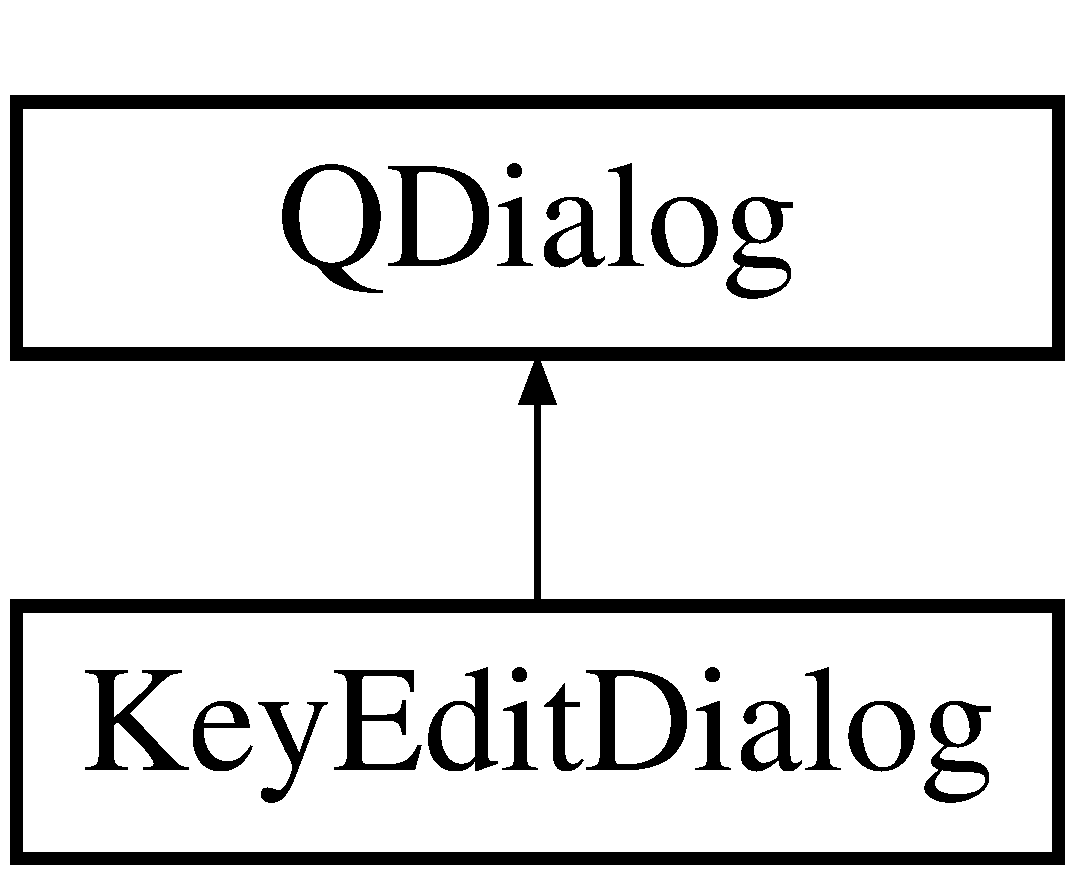
\includegraphics[height=2.000000cm]{class_key_edit_dialog}
\end{center}
\end{figure}
\subsection*{Signals}
\begin{DoxyCompactItemize}
\item 
\hyperlink{class_key_edit_dialog_a97e7fe242369a04650fea473fb1d68a4}{finish} (\hyperlink{class_key_element}{Key\+Element} $\ast$element)
\begin{DoxyCompactList}\small\item\em finish -\/ сигнал успешного завершения процесса создания \end{DoxyCompactList}\end{DoxyCompactItemize}
\subsection*{Public Member Functions}
\begin{DoxyCompactItemize}
\item 
\mbox{\Hypertarget{class_key_edit_dialog_ad71e9b9fec5ecb5fc89010dd17b60478}\label{class_key_edit_dialog_ad71e9b9fec5ecb5fc89010dd17b60478}} 
{\bfseries Key\+Edit\+Dialog} (Q\+Widget $\ast$parent=0)
\item 
void \hyperlink{class_key_edit_dialog_a88b517565674d5112be255d7f0808efe}{set\+Path} (Q\+Tree\+Widget\+Item $\ast$new\+Path)
\begin{DoxyCompactList}\small\item\em set\+Path -\/ установка адреса музыкального файла, с которым будет связан создаваемый объект \end{DoxyCompactList}\end{DoxyCompactItemize}


\subsection{Detailed Description}
\hyperlink{class_key_edit_dialog}{Key\+Edit\+Dialog} -\/ класс окна для назначения клавиш для музыкальных файлов и установки параметров их воспроизведения. таких как\+: Volume -\/ громкость музыкального файла, который будет воспроизводиться Repeating -\/ будет ли файл начинаться заново, когда он закончиться Key -\/ клавиша, к которой будет привязан музыкальный файл 

\subsection{Member Function Documentation}
\mbox{\Hypertarget{class_key_edit_dialog_a97e7fe242369a04650fea473fb1d68a4}\label{class_key_edit_dialog_a97e7fe242369a04650fea473fb1d68a4}} 
\index{Key\+Edit\+Dialog@{Key\+Edit\+Dialog}!finish@{finish}}
\index{finish@{finish}!Key\+Edit\+Dialog@{Key\+Edit\+Dialog}}
\subsubsection{\texorpdfstring{finish}{finish}}
{\footnotesize\ttfamily Key\+Edit\+Dialog\+::finish (\begin{DoxyParamCaption}\item[{\hyperlink{class_key_element}{Key\+Element} $\ast$}]{element }\end{DoxyParamCaption})\hspace{0.3cm}{\ttfamily [signal]}}



finish -\/ сигнал успешного завершения процесса создания 


\begin{DoxyParams}{Parameters}
{\em element} & -\/ результат создания объекта. Элемент с установленными параметрами \\
\hline
\end{DoxyParams}
\mbox{\Hypertarget{class_key_edit_dialog_a88b517565674d5112be255d7f0808efe}\label{class_key_edit_dialog_a88b517565674d5112be255d7f0808efe}} 
\index{Key\+Edit\+Dialog@{Key\+Edit\+Dialog}!set\+Path@{set\+Path}}
\index{set\+Path@{set\+Path}!Key\+Edit\+Dialog@{Key\+Edit\+Dialog}}
\subsubsection{\texorpdfstring{set\+Path()}{setPath()}}
{\footnotesize\ttfamily void Key\+Edit\+Dialog\+::set\+Path (\begin{DoxyParamCaption}\item[{Q\+Tree\+Widget\+Item $\ast$}]{new\+Path }\end{DoxyParamCaption})}



set\+Path -\/ установка адреса музыкального файла, с которым будет связан создаваемый объект 


\begin{DoxyParams}{Parameters}
{\em new\+Path} & -\/ адрес для установки \\
\hline
\end{DoxyParams}


The documentation for this class was generated from the following files\+:\begin{DoxyCompactItemize}
\item 
C\+:/\+Users/\+Alexey/\+Documents/\+Key\+Player3.\+x\+Rus/keyeditdialog.\+h\item 
C\+:/\+Users/\+Alexey/\+Documents/\+Key\+Player3.\+x\+Rus/keyeditdialog.\+cpp\end{DoxyCompactItemize}

\hypertarget{class_key_element}{}\section{Key\+Element Class Reference}
\label{class_key_element}\index{Key\+Element@{Key\+Element}}


\hyperlink{class_key_element}{Key\+Element} -\/ класс элемента, который хранит все параметры для воспроизведения музыкального файла. Таких как\+: адрес/клавиша/громкость/повторение  




{\ttfamily \#include $<$keyelement.\+h$>$}

Inheritance diagram for Key\+Element\+:\begin{figure}[H]
\begin{center}
\leavevmode
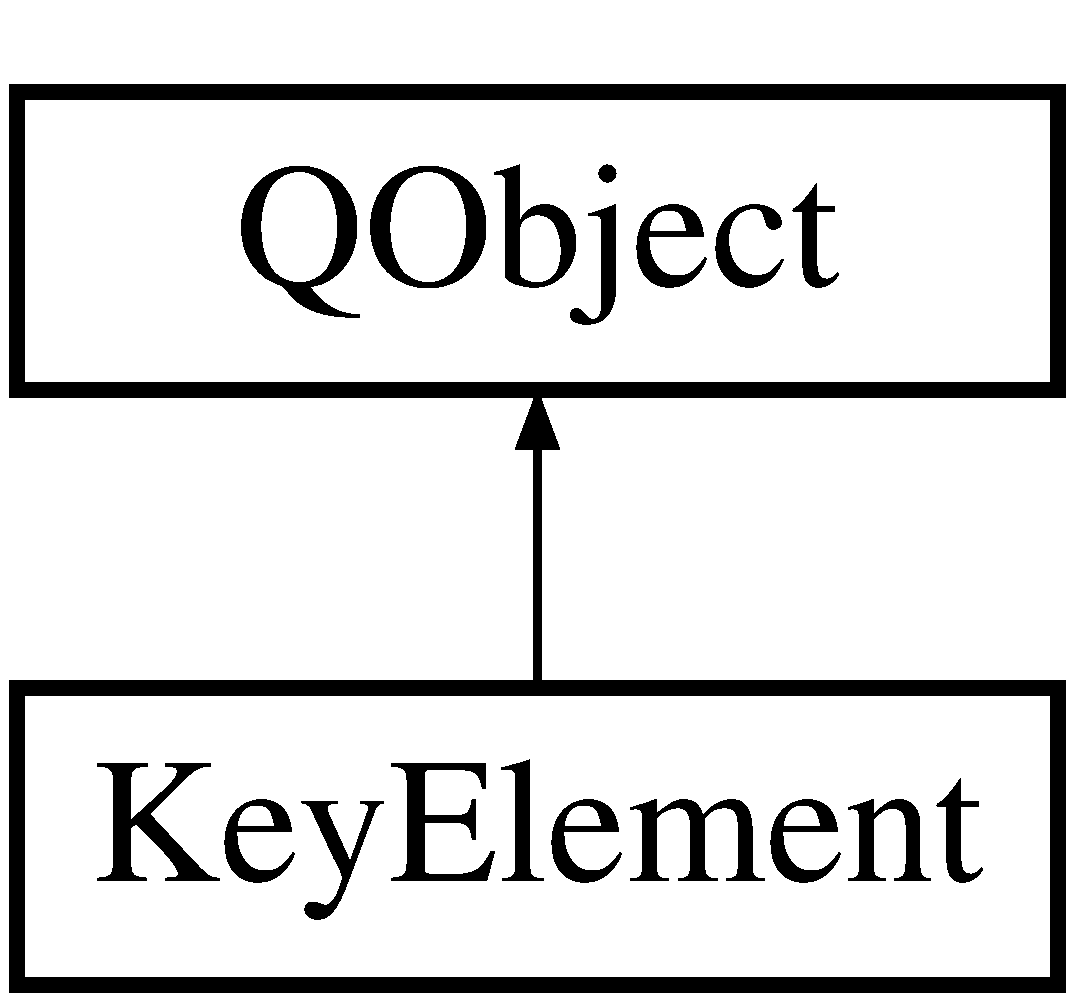
\includegraphics[height=2.000000cm]{class_key_element}
\end{center}
\end{figure}
\subsection*{Public Slots}
\begin{DoxyCompactItemize}
\item 
\mbox{\Hypertarget{class_key_element_aaaf9e68dd1d0456ba75b107542576161}\label{class_key_element_aaaf9e68dd1d0456ba75b107542576161}} 
void \hyperlink{class_key_element_aaaf9e68dd1d0456ba75b107542576161}{play} ()
\begin{DoxyCompactList}\small\item\em play -\/ запускает плеер \end{DoxyCompactList}\item 
\mbox{\Hypertarget{class_key_element_abeb24994e811465ee0e9ebd57bb83d18}\label{class_key_element_abeb24994e811465ee0e9ebd57bb83d18}} 
void \hyperlink{class_key_element_abeb24994e811465ee0e9ebd57bb83d18}{stop} ()
\begin{DoxyCompactList}\small\item\em stop -\/ останавливает плеер \end{DoxyCompactList}\item 
\mbox{\Hypertarget{class_key_element_a24e2928e97f101790f4f0c9bdfeced4c}\label{class_key_element_a24e2928e97f101790f4f0c9bdfeced4c}} 
void \hyperlink{class_key_element_a24e2928e97f101790f4f0c9bdfeced4c}{error\+Slot} ()
\begin{DoxyCompactList}\small\item\em error\+Slot -\/ слот ошибки, когда информация о файле загрузиться используется для проверки поддержки текущего файла плеером \end{DoxyCompactList}\end{DoxyCompactItemize}
\subsection*{Public Member Functions}
\begin{DoxyCompactItemize}
\item 
\mbox{\Hypertarget{class_key_element_a633b887fb11d894f467f4ab75eca4c06}\label{class_key_element_a633b887fb11d894f467f4ab75eca4c06}} 
{\bfseries Key\+Element} (Q\+Object $\ast$parent=0)
\item 
\hyperlink{class_key_element_aee0ae2b886fdc51944e3ea51d5f78162}{Key\+Element} (Q\+String name)
\begin{DoxyCompactList}\small\item\em \hyperlink{class_key_element}{Key\+Element} -\/ конструктор, в который передайтся алрес музыкального файла для связи \end{DoxyCompactList}\item 
Q\+Char \hyperlink{class_key_element_a6e0591a132b0b7c56196393552e7facd}{get\+Key} ()
\begin{DoxyCompactList}\small\item\em get\+Key получить клавишу, к которой привязан файл \end{DoxyCompactList}\item 
void \hyperlink{class_key_element_a19d376b834c91498ac136cf39ee31b5d}{set\+Key} (Q\+Char key)
\begin{DoxyCompactList}\small\item\em set\+Key -\/ установка клавиши, к которой будет привязан файл \end{DoxyCompactList}\item 
Q\+String \hyperlink{class_key_element_a30701d7ff9a6ab3ec4ac69c0487f462c}{get\+Name} ()
\begin{DoxyCompactList}\small\item\em get\+Name -\/ получить локальное имя музыкального файла \end{DoxyCompactList}\item 
Q\+String \hyperlink{class_key_element_a04460e1dedb060dd7c21a7a4ef3a3ee2}{get\+Path} ()
\begin{DoxyCompactList}\small\item\em get\+Path получить полный адрес музыкального файла \end{DoxyCompactList}\item 
int \hyperlink{class_key_element_ab9a05ec48e81319c0f9648535bf448ef}{get\+Format} ()
\begin{DoxyCompactList}\small\item\em get\+Format -\/ получить текущий статус музыкального файла \end{DoxyCompactList}\item 
void \hyperlink{class_key_element_aaee575ca9fabebd253806da9dcdc512f}{set\+Format} (int format)
\begin{DoxyCompactList}\small\item\em set\+Format -\/ установить текущий статус музыкального файла \end{DoxyCompactList}\item 
Q\+Tree\+Widget\+Item $\ast$ \hyperlink{class_key_element_aa4180885b87bb3eb0ed7418a96b79ffc}{get\+Item} ()
\begin{DoxyCompactList}\small\item\em get\+Item -\/ получить привязанный элемент из Q\+Tree\+Widget \end{DoxyCompactList}\item 
void \hyperlink{class_key_element_ab05c8efbfa5efad73e4e3b46d1521336}{set\+Item} (Q\+Tree\+Widget\+Item $\ast$item)
\begin{DoxyCompactList}\small\item\em set\+Item -\/ устанавливает связь с элементом из Q\+Tree\+Widget \end{DoxyCompactList}\item 
void \hyperlink{class_key_element_ae702f4dcd7becbce1737e6f4f3f69afe}{set\+Volume} (int volume)
\begin{DoxyCompactList}\small\item\em set\+Volume -\/ устанавливает громкость воспроизведения \end{DoxyCompactList}\item 
int \hyperlink{class_key_element_a088397040b8daccb6c7f5cd6cc8ef29f}{get\+Volume} ()
\begin{DoxyCompactList}\small\item\em get\+Volume -\/ получает текущее значение громкости \end{DoxyCompactList}\item 
Q\+Media\+Player $\ast$ \hyperlink{class_key_element_ae961bfbc0ce3eeb9b62ad12100ca977f}{get\+Player} ()
\begin{DoxyCompactList}\small\item\em get\+Player -\/ получает плеер воспроизведения текщего файла \end{DoxyCompactList}\item 
qint64 \hyperlink{class_key_element_a30c837b84299e75fcd41e0c6544d86ad}{duration} ()
\begin{DoxyCompactList}\small\item\em duration -\/ получает длительность музыкального файла (в мс) \end{DoxyCompactList}\item 
bool \hyperlink{class_key_element_ae4ec608b097cae6a325cbfc0d70ac01d}{is\+Valid} ()
\begin{DoxyCompactList}\small\item\em is\+Valid -\/ получает статус самого плеера. \end{DoxyCompactList}\item 
bool \hyperlink{class_key_element_a1b70040900c774127a3c1b6530e3374a}{is\+Repeated} ()
\begin{DoxyCompactList}\small\item\em is\+Repeated -\/ получает параметр повторения музыкального файла (при запуске с S\+H\+I\+FT) \end{DoxyCompactList}\item 
void \hyperlink{class_key_element_a3e9909b7a88b5bbba3b9fafe0d3a6652}{set\+Repeated} (bool repeat)
\begin{DoxyCompactList}\small\item\em set\+Repeated -\/ устанавливает параметр повторения музыкального файла (при запуске с S\+H\+I\+FT) \end{DoxyCompactList}\end{DoxyCompactItemize}


\subsection{Detailed Description}
\hyperlink{class_key_element}{Key\+Element} -\/ класс элемента, который хранит все параметры для воспроизведения музыкального файла. Таких как\+: адрес/клавиша/громкость/повторение 

\subsection{Constructor \& Destructor Documentation}
\mbox{\Hypertarget{class_key_element_aee0ae2b886fdc51944e3ea51d5f78162}\label{class_key_element_aee0ae2b886fdc51944e3ea51d5f78162}} 
\index{Key\+Element@{Key\+Element}!Key\+Element@{Key\+Element}}
\index{Key\+Element@{Key\+Element}!Key\+Element@{Key\+Element}}
\subsubsection{\texorpdfstring{Key\+Element()}{KeyElement()}}
{\footnotesize\ttfamily Key\+Element\+::\+Key\+Element (\begin{DoxyParamCaption}\item[{Q\+String}]{name }\end{DoxyParamCaption})}



\hyperlink{class_key_element}{Key\+Element} -\/ конструктор, в который передайтся алрес музыкального файла для связи 


\begin{DoxyParams}{Parameters}
{\em name} & -\/ адрес музыкального файла для создания связи \\
\hline
\end{DoxyParams}


\subsection{Member Function Documentation}
\mbox{\Hypertarget{class_key_element_a30c837b84299e75fcd41e0c6544d86ad}\label{class_key_element_a30c837b84299e75fcd41e0c6544d86ad}} 
\index{Key\+Element@{Key\+Element}!duration@{duration}}
\index{duration@{duration}!Key\+Element@{Key\+Element}}
\subsubsection{\texorpdfstring{duration()}{duration()}}
{\footnotesize\ttfamily qint64 Key\+Element\+::duration (\begin{DoxyParamCaption}{ }\end{DoxyParamCaption})}



duration -\/ получает длительность музыкального файла (в мс) 

\begin{DoxyReturn}{Returns}
-\/ длительность музыкального файла (в мс) 
\end{DoxyReturn}
\mbox{\Hypertarget{class_key_element_ab9a05ec48e81319c0f9648535bf448ef}\label{class_key_element_ab9a05ec48e81319c0f9648535bf448ef}} 
\index{Key\+Element@{Key\+Element}!get\+Format@{get\+Format}}
\index{get\+Format@{get\+Format}!Key\+Element@{Key\+Element}}
\subsubsection{\texorpdfstring{get\+Format()}{getFormat()}}
{\footnotesize\ttfamily int Key\+Element\+::get\+Format (\begin{DoxyParamCaption}{ }\end{DoxyParamCaption})}



get\+Format -\/ получить текущий статус музыкального файла 

\begin{DoxyReturn}{Returns}
-\/ код статуса\+: 0 -\/ в настоящий момент не проигрывается с помощью S\+H\+I\+FT 1 -\/ в настоящий момент проигрывается с помощью S\+H\+I\+FT 
\end{DoxyReturn}
\mbox{\Hypertarget{class_key_element_aa4180885b87bb3eb0ed7418a96b79ffc}\label{class_key_element_aa4180885b87bb3eb0ed7418a96b79ffc}} 
\index{Key\+Element@{Key\+Element}!get\+Item@{get\+Item}}
\index{get\+Item@{get\+Item}!Key\+Element@{Key\+Element}}
\subsubsection{\texorpdfstring{get\+Item()}{getItem()}}
{\footnotesize\ttfamily Q\+Tree\+Widget\+Item $\ast$ Key\+Element\+::get\+Item (\begin{DoxyParamCaption}{ }\end{DoxyParamCaption})}



get\+Item -\/ получить привязанный элемент из Q\+Tree\+Widget 

\begin{DoxyReturn}{Returns}
-\/ привязанный элемент из Q\+Tree\+Widget 
\end{DoxyReturn}
\mbox{\Hypertarget{class_key_element_a6e0591a132b0b7c56196393552e7facd}\label{class_key_element_a6e0591a132b0b7c56196393552e7facd}} 
\index{Key\+Element@{Key\+Element}!get\+Key@{get\+Key}}
\index{get\+Key@{get\+Key}!Key\+Element@{Key\+Element}}
\subsubsection{\texorpdfstring{get\+Key()}{getKey()}}
{\footnotesize\ttfamily Q\+Char Key\+Element\+::get\+Key (\begin{DoxyParamCaption}{ }\end{DoxyParamCaption})}



get\+Key получить клавишу, к которой привязан файл 

\begin{DoxyReturn}{Returns}
-\/ привязанная клавиша 
\end{DoxyReturn}
\mbox{\Hypertarget{class_key_element_a30701d7ff9a6ab3ec4ac69c0487f462c}\label{class_key_element_a30701d7ff9a6ab3ec4ac69c0487f462c}} 
\index{Key\+Element@{Key\+Element}!get\+Name@{get\+Name}}
\index{get\+Name@{get\+Name}!Key\+Element@{Key\+Element}}
\subsubsection{\texorpdfstring{get\+Name()}{getName()}}
{\footnotesize\ttfamily Q\+String Key\+Element\+::get\+Name (\begin{DoxyParamCaption}{ }\end{DoxyParamCaption})}



get\+Name -\/ получить локальное имя музыкального файла 

\begin{DoxyReturn}{Returns}
-\/ локальное имя файла 
\end{DoxyReturn}
\mbox{\Hypertarget{class_key_element_a04460e1dedb060dd7c21a7a4ef3a3ee2}\label{class_key_element_a04460e1dedb060dd7c21a7a4ef3a3ee2}} 
\index{Key\+Element@{Key\+Element}!get\+Path@{get\+Path}}
\index{get\+Path@{get\+Path}!Key\+Element@{Key\+Element}}
\subsubsection{\texorpdfstring{get\+Path()}{getPath()}}
{\footnotesize\ttfamily Q\+String Key\+Element\+::get\+Path (\begin{DoxyParamCaption}{ }\end{DoxyParamCaption})}



get\+Path получить полный адрес музыкального файла 

\begin{DoxyReturn}{Returns}
-\/ адрес файла 
\end{DoxyReturn}
\mbox{\Hypertarget{class_key_element_ae961bfbc0ce3eeb9b62ad12100ca977f}\label{class_key_element_ae961bfbc0ce3eeb9b62ad12100ca977f}} 
\index{Key\+Element@{Key\+Element}!get\+Player@{get\+Player}}
\index{get\+Player@{get\+Player}!Key\+Element@{Key\+Element}}
\subsubsection{\texorpdfstring{get\+Player()}{getPlayer()}}
{\footnotesize\ttfamily Q\+Media\+Player $\ast$ Key\+Element\+::get\+Player (\begin{DoxyParamCaption}{ }\end{DoxyParamCaption})}



get\+Player -\/ получает плеер воспроизведения текщего файла 

\begin{DoxyReturn}{Returns}
-\/ плеер воспроизведения 
\end{DoxyReturn}
\mbox{\Hypertarget{class_key_element_a088397040b8daccb6c7f5cd6cc8ef29f}\label{class_key_element_a088397040b8daccb6c7f5cd6cc8ef29f}} 
\index{Key\+Element@{Key\+Element}!get\+Volume@{get\+Volume}}
\index{get\+Volume@{get\+Volume}!Key\+Element@{Key\+Element}}
\subsubsection{\texorpdfstring{get\+Volume()}{getVolume()}}
{\footnotesize\ttfamily int Key\+Element\+::get\+Volume (\begin{DoxyParamCaption}{ }\end{DoxyParamCaption})}



get\+Volume -\/ получает текущее значение громкости 

\begin{DoxyReturn}{Returns}
-\/ значение громкости (от 0 до 100) 
\end{DoxyReturn}
\mbox{\Hypertarget{class_key_element_a1b70040900c774127a3c1b6530e3374a}\label{class_key_element_a1b70040900c774127a3c1b6530e3374a}} 
\index{Key\+Element@{Key\+Element}!is\+Repeated@{is\+Repeated}}
\index{is\+Repeated@{is\+Repeated}!Key\+Element@{Key\+Element}}
\subsubsection{\texorpdfstring{is\+Repeated()}{isRepeated()}}
{\footnotesize\ttfamily bool Key\+Element\+::is\+Repeated (\begin{DoxyParamCaption}{ }\end{DoxyParamCaption})}



is\+Repeated -\/ получает параметр повторения музыкального файла (при запуске с S\+H\+I\+FT) 

\begin{DoxyReturn}{Returns}
bool -\/ повторяется ли файл 
\end{DoxyReturn}
\mbox{\Hypertarget{class_key_element_ae4ec608b097cae6a325cbfc0d70ac01d}\label{class_key_element_ae4ec608b097cae6a325cbfc0d70ac01d}} 
\index{Key\+Element@{Key\+Element}!is\+Valid@{is\+Valid}}
\index{is\+Valid@{is\+Valid}!Key\+Element@{Key\+Element}}
\subsubsection{\texorpdfstring{is\+Valid()}{isValid()}}
{\footnotesize\ttfamily bool Key\+Element\+::is\+Valid (\begin{DoxyParamCaption}{ }\end{DoxyParamCaption})}



is\+Valid -\/ получает статус самого плеера. 

\begin{DoxyReturn}{Returns}
-\/ готов ли плеер к работе 
\end{DoxyReturn}
\mbox{\Hypertarget{class_key_element_aaee575ca9fabebd253806da9dcdc512f}\label{class_key_element_aaee575ca9fabebd253806da9dcdc512f}} 
\index{Key\+Element@{Key\+Element}!set\+Format@{set\+Format}}
\index{set\+Format@{set\+Format}!Key\+Element@{Key\+Element}}
\subsubsection{\texorpdfstring{set\+Format()}{setFormat()}}
{\footnotesize\ttfamily void Key\+Element\+::set\+Format (\begin{DoxyParamCaption}\item[{int}]{format }\end{DoxyParamCaption})}



set\+Format -\/ установить текущий статус музыкального файла 


\begin{DoxyParams}{Parameters}
{\em format} & -\/ код формата для установки 0 -\/ в настоящий момент не проигрывается с помощью S\+H\+I\+FT 1 -\/ в настоящий момент проигрывается с помощью S\+H\+I\+FT \\
\hline
\end{DoxyParams}
\mbox{\Hypertarget{class_key_element_ab05c8efbfa5efad73e4e3b46d1521336}\label{class_key_element_ab05c8efbfa5efad73e4e3b46d1521336}} 
\index{Key\+Element@{Key\+Element}!set\+Item@{set\+Item}}
\index{set\+Item@{set\+Item}!Key\+Element@{Key\+Element}}
\subsubsection{\texorpdfstring{set\+Item()}{setItem()}}
{\footnotesize\ttfamily void Key\+Element\+::set\+Item (\begin{DoxyParamCaption}\item[{Q\+Tree\+Widget\+Item $\ast$}]{item }\end{DoxyParamCaption})}



set\+Item -\/ устанавливает связь с элементом из Q\+Tree\+Widget 


\begin{DoxyParams}{Parameters}
{\em item} & -\/ элемент из Q\+Tree\+Widget для привязки \\
\hline
\end{DoxyParams}
\mbox{\Hypertarget{class_key_element_a19d376b834c91498ac136cf39ee31b5d}\label{class_key_element_a19d376b834c91498ac136cf39ee31b5d}} 
\index{Key\+Element@{Key\+Element}!set\+Key@{set\+Key}}
\index{set\+Key@{set\+Key}!Key\+Element@{Key\+Element}}
\subsubsection{\texorpdfstring{set\+Key()}{setKey()}}
{\footnotesize\ttfamily void Key\+Element\+::set\+Key (\begin{DoxyParamCaption}\item[{Q\+Char}]{key }\end{DoxyParamCaption})}



set\+Key -\/ установка клавиши, к которой будет привязан файл 


\begin{DoxyParams}{Parameters}
{\em key} & -\/ клавиша для привязки \\
\hline
\end{DoxyParams}
\mbox{\Hypertarget{class_key_element_a3e9909b7a88b5bbba3b9fafe0d3a6652}\label{class_key_element_a3e9909b7a88b5bbba3b9fafe0d3a6652}} 
\index{Key\+Element@{Key\+Element}!set\+Repeated@{set\+Repeated}}
\index{set\+Repeated@{set\+Repeated}!Key\+Element@{Key\+Element}}
\subsubsection{\texorpdfstring{set\+Repeated()}{setRepeated()}}
{\footnotesize\ttfamily void Key\+Element\+::set\+Repeated (\begin{DoxyParamCaption}\item[{bool}]{repeat }\end{DoxyParamCaption})}



set\+Repeated -\/ устанавливает параметр повторения музыкального файла (при запуске с S\+H\+I\+FT) 


\begin{DoxyParams}{Parameters}
{\em repeat} & -\/ будет ли файл повторяться \\
\hline
\end{DoxyParams}
\mbox{\Hypertarget{class_key_element_ae702f4dcd7becbce1737e6f4f3f69afe}\label{class_key_element_ae702f4dcd7becbce1737e6f4f3f69afe}} 
\index{Key\+Element@{Key\+Element}!set\+Volume@{set\+Volume}}
\index{set\+Volume@{set\+Volume}!Key\+Element@{Key\+Element}}
\subsubsection{\texorpdfstring{set\+Volume()}{setVolume()}}
{\footnotesize\ttfamily void Key\+Element\+::set\+Volume (\begin{DoxyParamCaption}\item[{int}]{volume }\end{DoxyParamCaption})}



set\+Volume -\/ устанавливает громкость воспроизведения 


\begin{DoxyParams}{Parameters}
{\em volume} & -\/ значение громкости (от 0 до 100) \\
\hline
\end{DoxyParams}


The documentation for this class was generated from the following files\+:\begin{DoxyCompactItemize}
\item 
C\+:/\+Users/\+Alexey/\+Documents/\+Key\+Player3.\+x\+Rus/keyelement.\+h\item 
C\+:/\+Users/\+Alexey/\+Documents/\+Key\+Player3.\+x\+Rus/keyelement.\+cpp\end{DoxyCompactItemize}

\hypertarget{class_key_main_window}{}\section{Key\+Main\+Window Class Reference}
\label{class_key_main_window}\index{Key\+Main\+Window@{Key\+Main\+Window}}


\hyperlink{class_key_main_window}{Key\+Main\+Window} -\/ класс главного окна с главным интерфейсом и с основной логикой  




{\ttfamily \#include $<$keymainwindow.\+h$>$}

Inheritance diagram for Key\+Main\+Window\+:\begin{figure}[H]
\begin{center}
\leavevmode
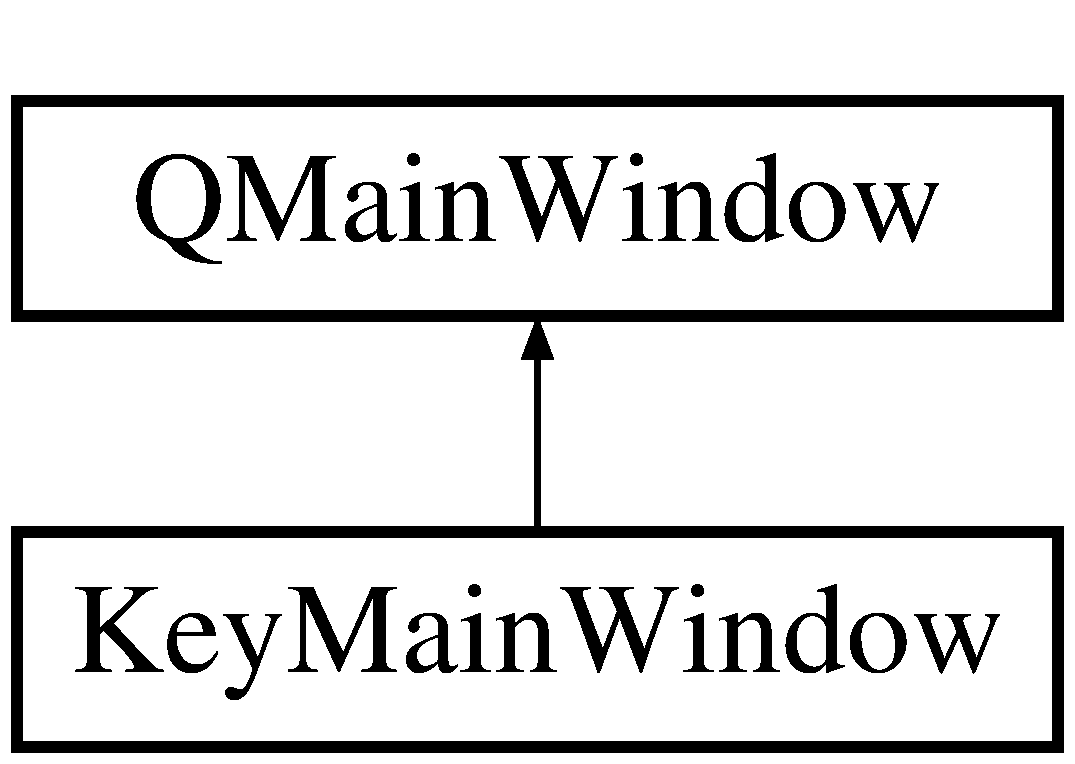
\includegraphics[height=2.000000cm]{class_key_main_window}
\end{center}
\end{figure}
\subsection*{Public Slots}
\begin{DoxyCompactItemize}
\item 
\mbox{\Hypertarget{class_key_main_window_a683dc7c13297f6f0bd3401ebfbf46e42}\label{class_key_main_window_a683dc7c13297f6f0bd3401ebfbf46e42}} 
void \hyperlink{class_key_main_window_a683dc7c13297f6f0bd3401ebfbf46e42}{on\+\_\+edit\+Button\+\_\+clicked} ()
\begin{DoxyCompactList}\small\item\em on\+\_\+edit\+Button\+\_\+clicked -\/ действие, которое выполниться при нажатии на кнопку \char`\"{}\+Edit\char`\"{} открывает окно для создания элемента плеера с выбранными параметрами. \end{DoxyCompactList}\item 
\mbox{\Hypertarget{class_key_main_window_a3e22453536f1a459df12248b5590c31b}\label{class_key_main_window_a3e22453536f1a459df12248b5590c31b}} 
void \hyperlink{class_key_main_window_a3e22453536f1a459df12248b5590c31b}{on\+\_\+add\+Button\+\_\+clicked} ()
\begin{DoxyCompactList}\small\item\em on\+\_\+add\+Button\+\_\+clicked -\/ действие, которое выполниться при нажатии на кнопку \char`\"{}\+Add\char`\"{} открывает окно проводника для выбора папки, содержащей музыкальные файлы (\char`\"{}$\ast$.\+mp3, $\ast$.\+wav\char`\"{}). \end{DoxyCompactList}\item 
\mbox{\Hypertarget{class_key_main_window_a5f4dc1cdd9398259fba83c17cf61ae53}\label{class_key_main_window_a5f4dc1cdd9398259fba83c17cf61ae53}} 
void \hyperlink{class_key_main_window_a5f4dc1cdd9398259fba83c17cf61ae53}{on\+\_\+delete\+Button\+\_\+clicked} ()
\begin{DoxyCompactList}\small\item\em on\+\_\+delete\+Button\+\_\+clicked -\/ действие, которое выполниться при нажатии на кнопку \char`\"{}\+Delete\char`\"{} удаляет выбранный элемент плеера из системы. \end{DoxyCompactList}\item 
\mbox{\Hypertarget{class_key_main_window_a2d07b299cbc4bf9550defad3ccbf0029}\label{class_key_main_window_a2d07b299cbc4bf9550defad3ccbf0029}} 
void \hyperlink{class_key_main_window_a2d07b299cbc4bf9550defad3ccbf0029}{on\+\_\+delete\+All\+Button\+\_\+clicked} ()
\begin{DoxyCompactList}\small\item\em on\+\_\+delete\+All\+Button\+\_\+clicked -\/ действие, которое выполниться при нажатии на кнопку \char`\"{}\+Delete all\char`\"{} удаляет все элементы плеера из всех слоёв. \end{DoxyCompactList}\item 
\mbox{\Hypertarget{class_key_main_window_a0b13e5083f4da72a98d710e0f1f41878}\label{class_key_main_window_a0b13e5083f4da72a98d710e0f1f41878}} 
void \hyperlink{class_key_main_window_a0b13e5083f4da72a98d710e0f1f41878}{on\+\_\+play\+Button\+\_\+clicked} ()
\begin{DoxyCompactList}\small\item\em on\+\_\+play\+Button\+\_\+clicked -\/ действие, которое выполниться при нажатии на кнопку \char`\"{}\+Play\char`\"{} открывает окно \hyperlink{class_play_window}{Play\+Window} и свзывает нажатия кнопок и клавиши в \hyperlink{class_play_window}{Play\+Window} с основной логической системой \end{DoxyCompactList}\item 
void \hyperlink{class_key_main_window_a13f36481d6b0d1f68dceca8a1c1ec2c1}{on\+\_\+file\+Tree\+Widget\+\_\+double\+Clicked} (const Q\+Model\+Index \&index)
\begin{DoxyCompactList}\small\item\em on\+\_\+file\+Tree\+Widget\+\_\+double\+Clicked -\/ действие, которое выполниться при двойном нажатии на элемент в Q\+Tree\+Widget ( = \char`\"{}\+Edit\char`\"{}) \end{DoxyCompactList}\item 
void \hyperlink{class_key_main_window_af82eadd35c704bc554d2465554dc48c0}{on\+\_\+key\+List\+Widget\+\_\+double\+Clicked} (const Q\+Model\+Index \&index)
\begin{DoxyCompactList}\small\item\em on\+\_\+key\+List\+Widget\+\_\+double\+Clicked -\/ действие, которое выполниться при двойном нажатии на элемент в Q\+List\+Widget \end{DoxyCompactList}\item 
void \hyperlink{class_key_main_window_a7a7856ea2f3e6d5bc6c4411057e64957}{start\+Play} (Q\+Char key)
\begin{DoxyCompactList}\small\item\em start\+Play -\/ начинает вопроизводить элемент плеера, связанный с данной клавишей \end{DoxyCompactList}\item 
void \hyperlink{class_key_main_window_a545142222ff293b73d57fb22ac6a122d}{stop\+Play} (Q\+Char key)
\begin{DoxyCompactList}\small\item\em stop\+Play -\/ останавливает воспроизведение элемента плеера, связанного с данной клавишей \end{DoxyCompactList}\item 
\mbox{\Hypertarget{class_key_main_window_a2fe2594084ecccb578c5991b8bf9844b}\label{class_key_main_window_a2fe2594084ecccb578c5991b8bf9844b}} 
void \hyperlink{class_key_main_window_a2fe2594084ecccb578c5991b8bf9844b}{stop\+All\+Play} ()
\begin{DoxyCompactList}\small\item\em stop\+All\+Play -\/ останавливает воспроизведение всех элементов плеера \end{DoxyCompactList}\item 
void \hyperlink{class_key_main_window_aaf05ff47462e7e4e396edc946a64fd7d}{edit\+Ok} (\hyperlink{class_key_element}{Key\+Element} $\ast$element)
\begin{DoxyCompactList}\small\item\em edit\+Ok -\/ слот, в который передаётся созданный элемент плеера для добавления в систему. \end{DoxyCompactList}\end{DoxyCompactItemize}
\subsection*{Public Member Functions}
\begin{DoxyCompactItemize}
\item 
\mbox{\Hypertarget{class_key_main_window_a91ed8b3bdc93749b0be61f28cffbb07a}\label{class_key_main_window_a91ed8b3bdc93749b0be61f28cffbb07a}} 
{\bfseries Key\+Main\+Window} (Q\+Widget $\ast$parent=0)
\item 
void \hyperlink{class_key_main_window_ac8658a2a9309909505bf6c0780919068}{add\+In\+List} (\hyperlink{class_key_element}{Key\+Element} $\ast$element)
\begin{DoxyCompactList}\small\item\em add\+In\+List -\/ добавляет элемент плеера в текущий список (keys, Q\+List\+Widget) \end{DoxyCompactList}\end{DoxyCompactItemize}


\subsection{Detailed Description}
\hyperlink{class_key_main_window}{Key\+Main\+Window} -\/ класс главного окна с главным интерфейсом и с основной логикой 

\subsection{Member Function Documentation}
\mbox{\Hypertarget{class_key_main_window_ac8658a2a9309909505bf6c0780919068}\label{class_key_main_window_ac8658a2a9309909505bf6c0780919068}} 
\index{Key\+Main\+Window@{Key\+Main\+Window}!add\+In\+List@{add\+In\+List}}
\index{add\+In\+List@{add\+In\+List}!Key\+Main\+Window@{Key\+Main\+Window}}
\subsubsection{\texorpdfstring{add\+In\+List()}{addInList()}}
{\footnotesize\ttfamily void Key\+Main\+Window\+::add\+In\+List (\begin{DoxyParamCaption}\item[{\hyperlink{class_key_element}{Key\+Element} $\ast$}]{element }\end{DoxyParamCaption})}



add\+In\+List -\/ добавляет элемент плеера в текущий список (keys, Q\+List\+Widget) 


\begin{DoxyParams}{Parameters}
{\em element} & -\/ элемент плеера для добавления \\
\hline
\end{DoxyParams}
\mbox{\Hypertarget{class_key_main_window_aaf05ff47462e7e4e396edc946a64fd7d}\label{class_key_main_window_aaf05ff47462e7e4e396edc946a64fd7d}} 
\index{Key\+Main\+Window@{Key\+Main\+Window}!edit\+Ok@{edit\+Ok}}
\index{edit\+Ok@{edit\+Ok}!Key\+Main\+Window@{Key\+Main\+Window}}
\subsubsection{\texorpdfstring{edit\+Ok}{editOk}}
{\footnotesize\ttfamily void Key\+Main\+Window\+::edit\+Ok (\begin{DoxyParamCaption}\item[{\hyperlink{class_key_element}{Key\+Element} $\ast$}]{element }\end{DoxyParamCaption})\hspace{0.3cm}{\ttfamily [slot]}}



edit\+Ok -\/ слот, в который передаётся созданный элемент плеера для добавления в систему. 


\begin{DoxyParams}{Parameters}
{\em element} & -\/ созданный элемент плеера добавляет созданный элемент плеера со всеми параметрами в Key\+List и Q\+List\+Widget \\
\hline
\end{DoxyParams}
\mbox{\Hypertarget{class_key_main_window_a13f36481d6b0d1f68dceca8a1c1ec2c1}\label{class_key_main_window_a13f36481d6b0d1f68dceca8a1c1ec2c1}} 
\index{Key\+Main\+Window@{Key\+Main\+Window}!on\+\_\+file\+Tree\+Widget\+\_\+double\+Clicked@{on\+\_\+file\+Tree\+Widget\+\_\+double\+Clicked}}
\index{on\+\_\+file\+Tree\+Widget\+\_\+double\+Clicked@{on\+\_\+file\+Tree\+Widget\+\_\+double\+Clicked}!Key\+Main\+Window@{Key\+Main\+Window}}
\subsubsection{\texorpdfstring{on\+\_\+file\+Tree\+Widget\+\_\+double\+Clicked}{on\_fileTreeWidget\_doubleClicked}}
{\footnotesize\ttfamily void Key\+Main\+Window\+::on\+\_\+file\+Tree\+Widget\+\_\+double\+Clicked (\begin{DoxyParamCaption}\item[{const Q\+Model\+Index \&}]{index }\end{DoxyParamCaption})\hspace{0.3cm}{\ttfamily [slot]}}



on\+\_\+file\+Tree\+Widget\+\_\+double\+Clicked -\/ действие, которое выполниться при двойном нажатии на элемент в Q\+Tree\+Widget ( = \char`\"{}\+Edit\char`\"{}) 


\begin{DoxyParams}{Parameters}
{\em index} & -\/ индекс текущего элемента открывает окно для создания элемента плеера с выбранными параметрами. \\
\hline
\end{DoxyParams}
\mbox{\Hypertarget{class_key_main_window_af82eadd35c704bc554d2465554dc48c0}\label{class_key_main_window_af82eadd35c704bc554d2465554dc48c0}} 
\index{Key\+Main\+Window@{Key\+Main\+Window}!on\+\_\+key\+List\+Widget\+\_\+double\+Clicked@{on\+\_\+key\+List\+Widget\+\_\+double\+Clicked}}
\index{on\+\_\+key\+List\+Widget\+\_\+double\+Clicked@{on\+\_\+key\+List\+Widget\+\_\+double\+Clicked}!Key\+Main\+Window@{Key\+Main\+Window}}
\subsubsection{\texorpdfstring{on\+\_\+key\+List\+Widget\+\_\+double\+Clicked}{on\_keyListWidget\_doubleClicked}}
{\footnotesize\ttfamily void Key\+Main\+Window\+::on\+\_\+key\+List\+Widget\+\_\+double\+Clicked (\begin{DoxyParamCaption}\item[{const Q\+Model\+Index \&}]{index }\end{DoxyParamCaption})\hspace{0.3cm}{\ttfamily [slot]}}



on\+\_\+key\+List\+Widget\+\_\+double\+Clicked -\/ действие, которое выполниться при двойном нажатии на элемент в Q\+List\+Widget 


\begin{DoxyParams}{Parameters}
{\em index} & -\/ индекс текущего элемента воспроизведение текущего жлемента плеера, либо его остановка. \\
\hline
\end{DoxyParams}
\mbox{\Hypertarget{class_key_main_window_a7a7856ea2f3e6d5bc6c4411057e64957}\label{class_key_main_window_a7a7856ea2f3e6d5bc6c4411057e64957}} 
\index{Key\+Main\+Window@{Key\+Main\+Window}!start\+Play@{start\+Play}}
\index{start\+Play@{start\+Play}!Key\+Main\+Window@{Key\+Main\+Window}}
\subsubsection{\texorpdfstring{start\+Play}{startPlay}}
{\footnotesize\ttfamily void Key\+Main\+Window\+::start\+Play (\begin{DoxyParamCaption}\item[{Q\+Char}]{key }\end{DoxyParamCaption})\hspace{0.3cm}{\ttfamily [slot]}}



start\+Play -\/ начинает вопроизводить элемент плеера, связанный с данной клавишей 


\begin{DoxyParams}{Parameters}
{\em key} & -\/ код символа, который был активирован\+: \textquotesingle{}0\textquotesingle{} -\/ \textquotesingle{}9\textquotesingle{} -\/ переход к другому слою \textquotesingle{}a\textquotesingle{} -\/ \textquotesingle{}z\textquotesingle{} -\/ клавиши \textquotesingle{}.\textquotesingle{} -\/ S\+H\+I\+FT \\
\hline
\end{DoxyParams}
\mbox{\Hypertarget{class_key_main_window_a545142222ff293b73d57fb22ac6a122d}\label{class_key_main_window_a545142222ff293b73d57fb22ac6a122d}} 
\index{Key\+Main\+Window@{Key\+Main\+Window}!stop\+Play@{stop\+Play}}
\index{stop\+Play@{stop\+Play}!Key\+Main\+Window@{Key\+Main\+Window}}
\subsubsection{\texorpdfstring{stop\+Play}{stopPlay}}
{\footnotesize\ttfamily void Key\+Main\+Window\+::stop\+Play (\begin{DoxyParamCaption}\item[{Q\+Char}]{key }\end{DoxyParamCaption})\hspace{0.3cm}{\ttfamily [slot]}}



stop\+Play -\/ останавливает воспроизведение элемента плеера, связанного с данной клавишей 


\begin{DoxyParams}{Parameters}
{\em key} & -\/ код символа, который был активирован\+: \textquotesingle{}a\textquotesingle{} -\/ \textquotesingle{}z\textquotesingle{} -\/ клавиши \textquotesingle{}.\textquotesingle{} -\/ S\+H\+I\+FT \\
\hline
\end{DoxyParams}


The documentation for this class was generated from the following files\+:\begin{DoxyCompactItemize}
\item 
C\+:/\+Users/\+Alexey/\+Documents/\+Key\+Player3.\+x\+Rus/keymainwindow.\+h\item 
C\+:/\+Users/\+Alexey/\+Documents/\+Key\+Player3.\+x\+Rus/keymainwindow.\+cpp\end{DoxyCompactItemize}

\hypertarget{class_play_window}{}\section{Play\+Window Class Reference}
\label{class_play_window}\index{Play\+Window@{Play\+Window}}


The \hyperlink{class_play_window}{Play\+Window} класс окна свиртуальной клавиатурой. Отправляет сигналы при нажатии/отпускании клавиш главному окну  




{\ttfamily \#include $<$playwindow.\+h$>$}

Inheritance diagram for Play\+Window\+:\begin{figure}[H]
\begin{center}
\leavevmode
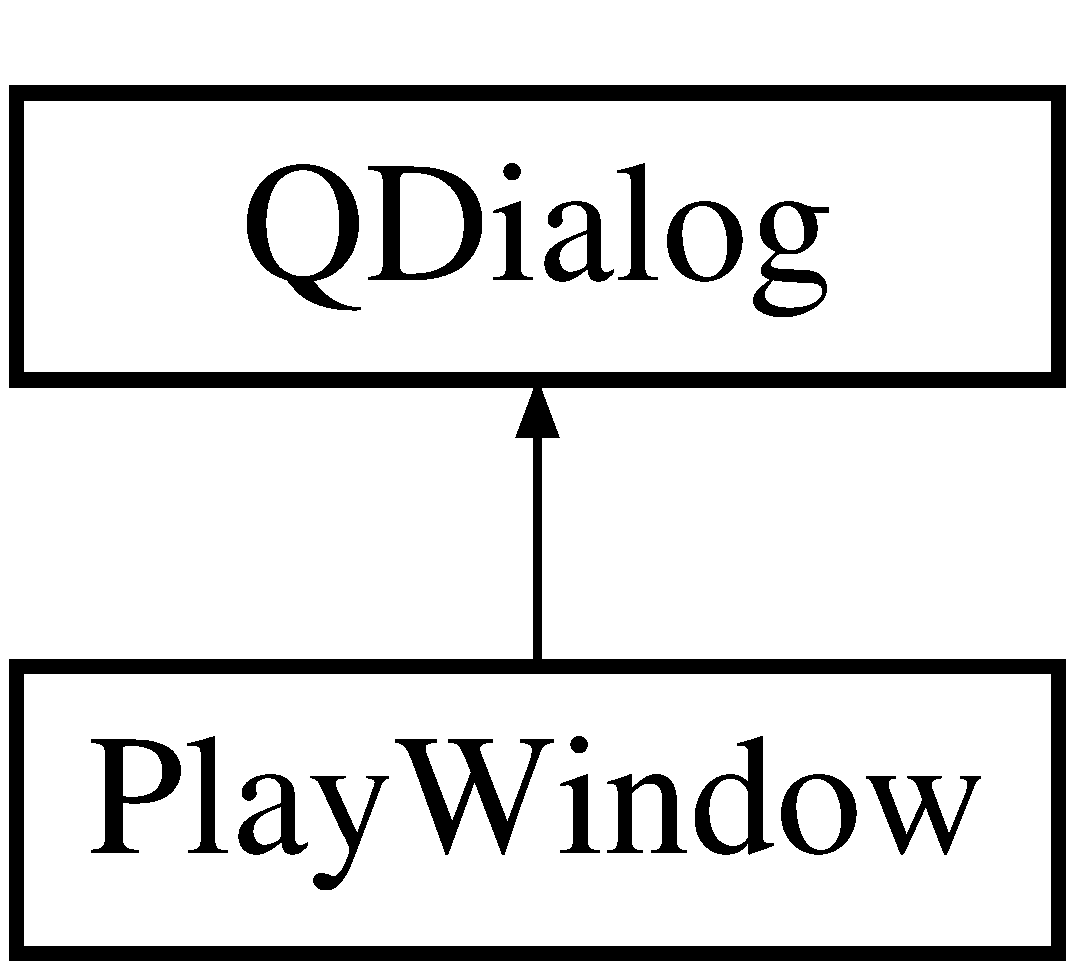
\includegraphics[height=2.000000cm]{class_play_window}
\end{center}
\end{figure}
\subsection*{Signals}
\begin{DoxyCompactItemize}
\item 
void \hyperlink{class_play_window_ae629638312cf77e32ca2d681988f67bb}{button\+Pressed\+Signal} (Q\+Char key)
\begin{DoxyCompactList}\small\item\em button\+Pressed\+Signal -\/ сигнал, передаваемый, когда какая-\/либо клавиша была нажата \end{DoxyCompactList}\item 
void \hyperlink{class_play_window_a4cc0e9d4e067da86aaf025c2863da5d6}{button\+Released\+Signal} (Q\+Char key)
\begin{DoxyCompactList}\small\item\em button\+Released\+Signal -\/ сигнал, передаваемый, когда какая-\/либо клавиша была отпущена \end{DoxyCompactList}\end{DoxyCompactItemize}
\subsection*{Public Member Functions}
\begin{DoxyCompactItemize}
\item 
\mbox{\Hypertarget{class_play_window_ad88fb98822ab0c52b76e4005dfd10647}\label{class_play_window_ad88fb98822ab0c52b76e4005dfd10647}} 
{\bfseries Play\+Window} (Q\+Widget $\ast$parent=0)
\end{DoxyCompactItemize}
\subsection*{Protected Member Functions}
\begin{DoxyCompactItemize}
\item 
void \hyperlink{class_play_window_aa931ee4edcea15ecb535c45db914fd83}{key\+Press\+Event} (Q\+Key\+Event $\ast$event)
\begin{DoxyCompactList}\small\item\em key\+Press\+Event -\/ метод обработки нажатии какой-\/либо клавиши \end{DoxyCompactList}\item 
void \hyperlink{class_play_window_a0812a60414cc058a491d65b9ed919f5f}{key\+Release\+Event} (Q\+Key\+Event $\ast$event)
\begin{DoxyCompactList}\small\item\em key\+Release\+Event -\/ метод обработки отпускания какой-\/либо клавиши \end{DoxyCompactList}\end{DoxyCompactItemize}


\subsection{Detailed Description}
The \hyperlink{class_play_window}{Play\+Window} класс окна свиртуальной клавиатурой. Отправляет сигналы при нажатии/отпускании клавиш главному окну 

\subsection{Member Function Documentation}
\mbox{\Hypertarget{class_play_window_ae629638312cf77e32ca2d681988f67bb}\label{class_play_window_ae629638312cf77e32ca2d681988f67bb}} 
\index{Play\+Window@{Play\+Window}!button\+Pressed\+Signal@{button\+Pressed\+Signal}}
\index{button\+Pressed\+Signal@{button\+Pressed\+Signal}!Play\+Window@{Play\+Window}}
\subsubsection{\texorpdfstring{button\+Pressed\+Signal}{buttonPressedSignal}}
{\footnotesize\ttfamily void Play\+Window\+::button\+Pressed\+Signal (\begin{DoxyParamCaption}\item[{Q\+Char}]{key }\end{DoxyParamCaption})\hspace{0.3cm}{\ttfamily [signal]}}



button\+Pressed\+Signal -\/ сигнал, передаваемый, когда какая-\/либо клавиша была нажата 


\begin{DoxyParams}{Parameters}
{\em key} & -\/ код клавиши, которая была нажата \\
\hline
\end{DoxyParams}
\mbox{\Hypertarget{class_play_window_a4cc0e9d4e067da86aaf025c2863da5d6}\label{class_play_window_a4cc0e9d4e067da86aaf025c2863da5d6}} 
\index{Play\+Window@{Play\+Window}!button\+Released\+Signal@{button\+Released\+Signal}}
\index{button\+Released\+Signal@{button\+Released\+Signal}!Play\+Window@{Play\+Window}}
\subsubsection{\texorpdfstring{button\+Released\+Signal}{buttonReleasedSignal}}
{\footnotesize\ttfamily void Play\+Window\+::button\+Released\+Signal (\begin{DoxyParamCaption}\item[{Q\+Char}]{key }\end{DoxyParamCaption})\hspace{0.3cm}{\ttfamily [signal]}}



button\+Released\+Signal -\/ сигнал, передаваемый, когда какая-\/либо клавиша была отпущена 


\begin{DoxyParams}{Parameters}
{\em key} & -\/ код клавиши, которая была отпущена \\
\hline
\end{DoxyParams}
\mbox{\Hypertarget{class_play_window_aa931ee4edcea15ecb535c45db914fd83}\label{class_play_window_aa931ee4edcea15ecb535c45db914fd83}} 
\index{Play\+Window@{Play\+Window}!key\+Press\+Event@{key\+Press\+Event}}
\index{key\+Press\+Event@{key\+Press\+Event}!Play\+Window@{Play\+Window}}
\subsubsection{\texorpdfstring{key\+Press\+Event()}{keyPressEvent()}}
{\footnotesize\ttfamily void Play\+Window\+::key\+Press\+Event (\begin{DoxyParamCaption}\item[{Q\+Key\+Event $\ast$}]{event }\end{DoxyParamCaption})\hspace{0.3cm}{\ttfamily [protected]}}



key\+Press\+Event -\/ метод обработки нажатии какой-\/либо клавиши 


\begin{DoxyParams}{Parameters}
{\em event} & -\/ событие нажатия отправляет сигнал главному окну и отображает состояние клавиатуры на виртуальной клавиатуре \\
\hline
\end{DoxyParams}
\mbox{\Hypertarget{class_play_window_a0812a60414cc058a491d65b9ed919f5f}\label{class_play_window_a0812a60414cc058a491d65b9ed919f5f}} 
\index{Play\+Window@{Play\+Window}!key\+Release\+Event@{key\+Release\+Event}}
\index{key\+Release\+Event@{key\+Release\+Event}!Play\+Window@{Play\+Window}}
\subsubsection{\texorpdfstring{key\+Release\+Event()}{keyReleaseEvent()}}
{\footnotesize\ttfamily void Play\+Window\+::key\+Release\+Event (\begin{DoxyParamCaption}\item[{Q\+Key\+Event $\ast$}]{event }\end{DoxyParamCaption})\hspace{0.3cm}{\ttfamily [protected]}}



key\+Release\+Event -\/ метод обработки отпускания какой-\/либо клавиши 


\begin{DoxyParams}{Parameters}
{\em event} & -\/ событие отпускания отправляет сигнал главному окну и отображает состояние клавиатуры на виртуальной клавиатуре \\
\hline
\end{DoxyParams}


The documentation for this class was generated from the following files\+:\begin{DoxyCompactItemize}
\item 
C\+:/\+Users/\+Alexey/\+Documents/\+Key\+Player3.\+x\+Rus/playwindow.\+h\item 
C\+:/\+Users/\+Alexey/\+Documents/\+Key\+Player3.\+x\+Rus/playwindow.\+cpp\end{DoxyCompactItemize}

\hypertarget{class_try_player}{}\section{Try\+Player Class Reference}
\label{class_try_player}\index{Try\+Player@{Try\+Player}}


\hyperlink{class_try_player}{Try\+Player} -\/ класс для проверки поддержки музыкальных фалов, когда файлы были добавлены в Q\+Tree\+Widget. Уничтожает сам себя  




{\ttfamily \#include $<$tryplayer.\+h$>$}

Inheritance diagram for Try\+Player\+:\begin{figure}[H]
\begin{center}
\leavevmode
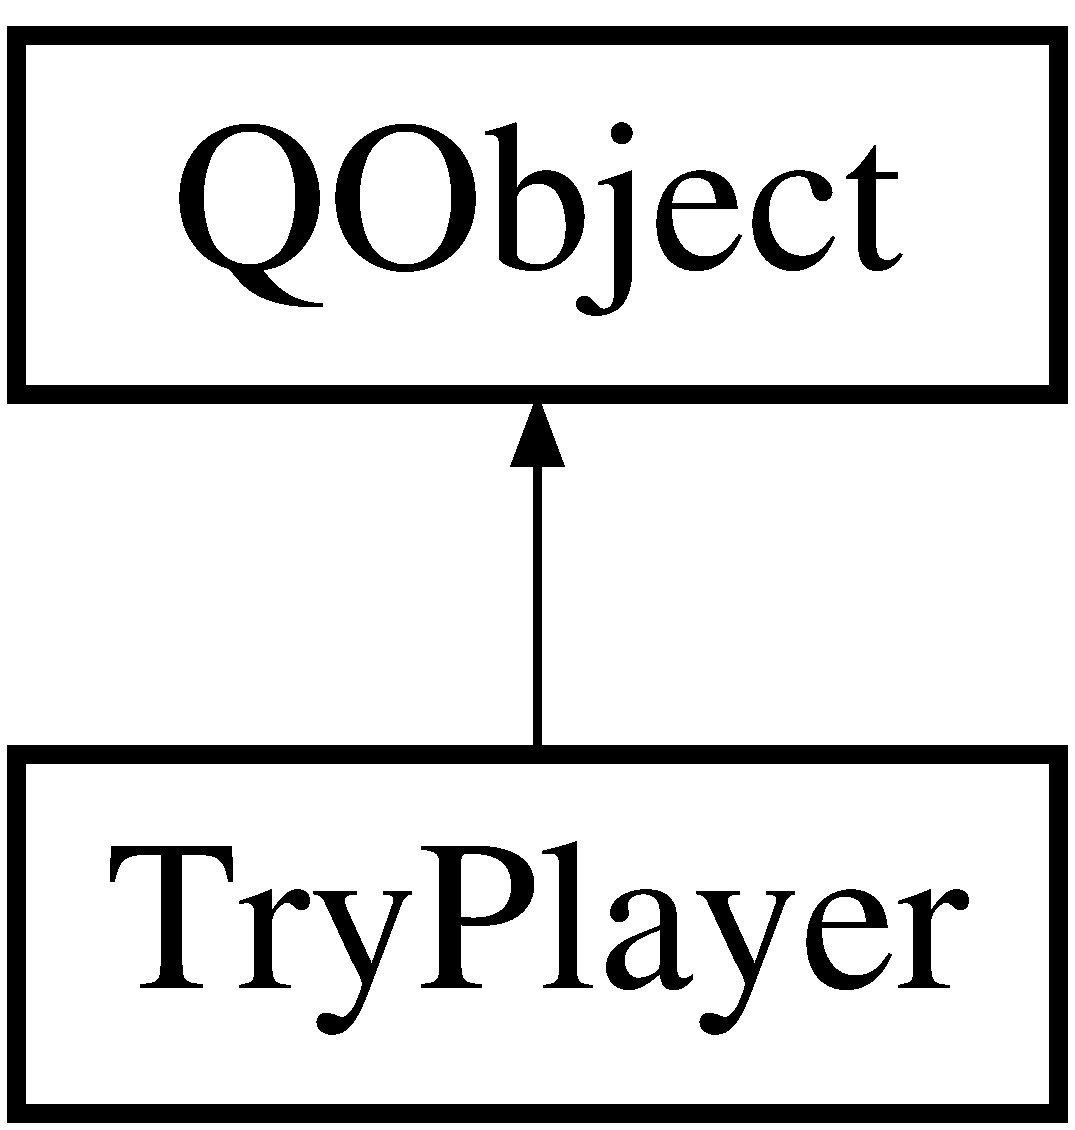
\includegraphics[height=2.000000cm]{class_try_player}
\end{center}
\end{figure}
\subsection*{Public Slots}
\begin{DoxyCompactItemize}
\item 
\mbox{\Hypertarget{class_try_player_a67d1caa173bb754d46daaa03111f6d84}\label{class_try_player_a67d1caa173bb754d46daaa03111f6d84}} 
void \hyperlink{class_try_player_a67d1caa173bb754d46daaa03111f6d84}{duration\+Changed\+Slot} ()
\begin{DoxyCompactList}\small\item\em duration\+Changed\+Slot -\/ слот, который активируется тогда, когда была загружена длительность выбранного файла \end{DoxyCompactList}\item 
\mbox{\Hypertarget{class_try_player_ad4a2fdf909def192746ace6cc83cb1e1}\label{class_try_player_ad4a2fdf909def192746ace6cc83cb1e1}} 
void \hyperlink{class_try_player_ad4a2fdf909def192746ace6cc83cb1e1}{error\+Slot} ()
\begin{DoxyCompactList}\small\item\em error\+Slot -\/ слот, который активируется тогда, когда инормация о музыкальном файле была загружена некорректно. \end{DoxyCompactList}\end{DoxyCompactItemize}
\subsection*{Public Member Functions}
\begin{DoxyCompactItemize}
\item 
\mbox{\Hypertarget{class_try_player_a04f52a541353910e794c4605b5c39376}\label{class_try_player_a04f52a541353910e794c4605b5c39376}} 
{\bfseries Try\+Player} (Q\+Object $\ast$parent=0)
\item 
\hyperlink{class_try_player_a300f8dd127a92e0b1d1bc8bf75bf979a}{Try\+Player} (Q\+Tree\+Widget\+Item $\ast$item)
\begin{DoxyCompactList}\small\item\em \hyperlink{class_try_player}{Try\+Player} -\/ создаёт самоуничтожающийся объект \hyperlink{class_try_player}{Try\+Player}, с выбранным файлом \end{DoxyCompactList}\end{DoxyCompactItemize}


\subsection{Detailed Description}
\hyperlink{class_try_player}{Try\+Player} -\/ класс для проверки поддержки музыкальных фалов, когда файлы были добавлены в Q\+Tree\+Widget. Уничтожает сам себя 

\subsection{Constructor \& Destructor Documentation}
\mbox{\Hypertarget{class_try_player_a300f8dd127a92e0b1d1bc8bf75bf979a}\label{class_try_player_a300f8dd127a92e0b1d1bc8bf75bf979a}} 
\index{Try\+Player@{Try\+Player}!Try\+Player@{Try\+Player}}
\index{Try\+Player@{Try\+Player}!Try\+Player@{Try\+Player}}
\subsubsection{\texorpdfstring{Try\+Player()}{TryPlayer()}}
{\footnotesize\ttfamily Try\+Player\+::\+Try\+Player (\begin{DoxyParamCaption}\item[{Q\+Tree\+Widget\+Item $\ast$}]{item }\end{DoxyParamCaption})}



\hyperlink{class_try_player}{Try\+Player} -\/ создаёт самоуничтожающийся объект \hyperlink{class_try_player}{Try\+Player}, с выбранным файлом 


\begin{DoxyParams}{Parameters}
{\em item} & -\/ элемент Q\+Tree\+Widget для проверки \\
\hline
\end{DoxyParams}


The documentation for this class was generated from the following files\+:\begin{DoxyCompactItemize}
\item 
C\+:/\+Users/\+Alexey/\+Documents/\+Key\+Player3.\+x\+Rus/tryplayer.\+h\item 
C\+:/\+Users/\+Alexey/\+Documents/\+Key\+Player3.\+x\+Rus/tryplayer.\+cpp\end{DoxyCompactItemize}

%--- End generated contents ---

% Index
\backmatter
\newpage
\phantomsection
\clearemptydoublepage
\addcontentsline{toc}{chapter}{Index}
\printindex

\end{document}
